\documentclass[a4paper, 12pt]{article}

% basic package list
%\usepackage[T1]{fontenc}
\usepackage{fontspec}
\defaultfontfeatures{Mapping=tex-text}
\usepackage[margin=25mm]{geometry}
\usepackage{amsmath}
\usepackage{amsfonts}
\usepackage{amssymb}
\usepackage{graphicx}

% other packages
\usepackage{xunicode}
\usepackage{xltxtra}
\usepackage{hyperref}         % hyperlinks
\usepackage{booktabs}         % professional-quality tables
\usepackage{indentfirst}      % to indent section first paragraph
\usepackage{url}              % simple URL typesetting
\usepackage{natbib}
\usepackage[modulo]{lineno}
\usepackage{sectsty}          % to change section font size
\usepackage[flushleft]{threeparttable} % table with note
\usepackage{mathtools}
\usepackage{indentfirst}
\usepackage{multirow}
\usepackage[labelfont=bf]{caption}
\usepackage{lineno}
\usepackage{courier}


% black hypelinks with no border
\hypersetup{
    colorlinks,
    citecolor=black,
    filecolor=black,
    linkcolor=black,
    urlcolor=black
}

% set additional parameters
\setcitestyle{authoryear,open={(},close={)}}
\graphicspath {{Figures/}}

\sectionfont{\fontsize{14}{19}\selectfont}
\subsectionfont{\fontsize{12}{17}\selectfont}

\renewcommand{\thefigure}{S\arabic{figure}}
\renewcommand{\thetable}{S\arabic{table}}

\setcounter{figure}{0}

% reduce page number font size
\renewcommand*{\thepage}{\footnotesize\arabic{page}}

\title{Supplementary Material for: Joint inference of adaptive and demographic history from temporal population genomic data}
\author{\small
            Vitor A. C. Pavinato$^{1,2,3}$, Stéphane De Mita$^4$, Jean-Michel Marin$^2$, Miguel de Navascués$^{1,5*}$}
\date{{\footnotesize %
    $^1$CBGP, INRAE, CIRAD, IRD, Montpellier SupAgro, Université de Montpellier, Montpellier, France\\%
    $^2$UMR Institut Montpelliérain Alexander Grothendieck, Université de Montpellier, France\\%  
    $^3$Entomology Dept., CFAES, The Ohio State University, Wooster, USA\\%
    $^4$UMR Interactions Arbres-Microorganismes, INRAE, France \\%
    $^5$Human Evolution, Department of Organismal Biology, Uppsala University, Uppsala, Sweden\\%  
    $^*$corresponding author: miguel.navascues@inrae.fr\\[2ex]%
    }
    \footnotesize\today    
}
\begin{document}
\maketitle

\newpage

\section*{S1 Supplementary Table}

\begin{table}[ht]
 \caption{\textbf{Notation.}}
  \centering
  \label{table:tableS1}
  \begin{tabular}{ll}
   \cmidrule(r){1-2}
    Symbol                  & Meaning \\
    \midrule
    $c_{\mathrm{0}}$        & recombination rate per base pair per generation \\
    $G$                     & genome size\\
    $h$                     & dominance coefficient\\
    $L$                     & mean substitution load\\
    $N$                     & population size during the inference period\\ 
    $N_{\mathrm{0}}$        & population size during the burn-in period\\
    $N_{\mathrm{e}}$        & effective population size during the inference period\\
    $P_{\mathrm{R}}$        & proportion of non-neutral regions\\
    $P_{\mathrm{B}}$        & proportion of beneficial mutations per non-neutral region\\
    $P$                     & proportion of polymorphisms under strong selection, i.e. $s > 1/ N_{\mathrm{e}}$\\
    $s$                     & selection coefficient\\
    $\bar{s}$               & average selection coefficients of mutations under strong selection\\
    $t_1$ and $t_2$         & generations were samples of individuals were taken\\
    $W_{\mathrm{max}i}$     & fitness of individual with highest fitness in the population in generation $i$\\
    $\bar{W_{i}}$           & mean fitness of the population in generation $i$\\
    $\gamma$                & mean of the gamma distribution where the selection coefficients of each\\
                            & beneficial mutation was sampled\\
    $\mu$                   & mutation rate per generation\\
    $\mu_{\mathrm{b}}$      & mutation rate of beneficial mutations per generation\\
    $\tau$                  & length of time-interval between the first and the second sample\\
    $\theta_{\mathrm{b}}$   & scaled mutation rate of beneficial mutations\\
&\\
    
    \bottomrule
  \end{tabular}
  \label{tab:supple_symbols}
\end{table}

\section*{S2 Supplementary Methods}

\subsection*{S2.1 List of summary statistics}

Three groups of summary statistics were calculated for the reference table (\texttt{e.g} training data): 1) summary statistics calculated SNP-by-SNPs (i.e. locus-specific summary statistics - LSS); 2) summary statistics calculated for nucleotide sequence (i.e. window summary statistics - WSS) - in this case a window containing base positions was defined around each SNP in the dataset; and 3) summary statistics calculated globally by averaging the locus-specific or window-specific summary statistics (global summary statistics - GSS). Summary statistics informative about within-population diversity as $H_{\mathrm{E}}$ were calculated for each time point individually and marginally by pooling all individuals sampled together. For the summary statistics calculated in a window, three window sizes were used: 500bp, 5Kbp, and 10Kbp. For the site-frequency spectrum, the allele counts were used instead of frequency, and all bins were included in the reference table.

\begin{enumerate}
	\item LSSs - Locus-specific summary statistics:
    \begin{enumerate}
    	\item $D_{\mathrm{j}}$ - Jost's $D$ \citep{Jost:2008cs,Jost:2009hn};
        \item $F_{\mathrm{ST}}$ - Weir and Cockerham's $F_{\mathrm{ST}}$ \citep{Weir:1984dx};
        \item $H_{\mathrm{E}}$ - Expected Heterozygosity;
    \end{enumerate}
    \item WSSs - Window-specific summary statistics (window sizes - 500bp, 5Kbp and 10Kbp):
    \begin{enumerate}
        \item $D_{\mathrm{j}}$ - Jost's $D$;
        \item $F_{\mathrm{ST}}$ - Weir and Cockerham's $F_{\mathrm{ST}}$;
        \item $D_{\mathrm{a}}$ - Net distance between populations;
        \item $H_{\mathrm{E}}$ - Expected Heterozygosity;
        \item $S$ - Number of polymorphic sites;
        \item $\pi$ - Nucleotide diversity \citep{Nei:1979uk};
        \item $\theta_{\mathrm{W}}$ - Watterson's 4Nu estimator \citep{Watterson:1975bh};
        \item $T_{\mathrm{j}}D$ - Tajima's D \citep{Tajima:1989un};
    \end{enumerate}
    \item Global summary statistics:
    \begin{enumerate}
        \item All summary statistics enumerated above (including the within population calculations);
        \item SFS bins - binned Joint Site-frequency spectrum $SFS$ \citep{Ewing:2016gv};
        \item mean, variance, kurtosis, skewness and the 5\% and 95\% quantiles of all intra-locus summary statistics presented above (LSSs and WSSs);
    \end{enumerate}
\end{enumerate}

\section*{S3 Supplementary Results}

\subsection*{S3.1 ABC-RF}

Figure~\ref{fig:supple_pods_priors} shows the prior distribution of the parameters and latent variables that were estimated with the ABC-RF. These distributions correspond to the values that were used to train ABC-Random forests. 

Figure~\ref{fig:supple_oob_sel} shows the distribution of Random Forest OOB estimates on the observed values (the ones used to train the RF) for model parameters and other latent variables informative about selection. The ABC-RF regressions performed poorly on the inference of two parameters of the selection dynamics $P_{\mathrm{R}}P_{\mathrm{B}}$ and $\gamma$. On the other hand, the ABC-RF performed better on the latent variables $P$, and $\bar{s}$ (which can be viewed as the realization of the two aforementioned parameters). Each value of these latent variables was obtained from the simulation by 1) calculating the relative proportion of strongly beneficial mutations (those with $s > 1/N_{\mathrm{e}}$) over all segregating mutations, 2) averaging their $s$ values. 
The estimation of substitution load $L$ had also somehow good performance. It performed well for higher values but poorly for lower values, as we can see in the distribution of the estimated OOB values against the true values (Figure~\ref{fig:supple_oob_sel} e). It seems that only strong adaptive dynamics (many loci under selection or strong selection) leaves a polymoprhism patterns that are informative about substitution load. The proportion of strongly beneficial mutations that segregated in the population, $P$ can also be used as a complementary estimator to characterize the adaptive dynamics (it is complementary to $\theta_{\mathrm{b}}$ presented in the main text). 

Figure~\ref{fig:supple_oob_demo} also presents the distribution OOB estimates with the true observed values for model parameters and for the latent variables informative about drift. For these model parameters, ABC-RF could not satisfactory recover the recombination rate $c_{\mathrm{0}}$ as expected given the summary statistics calculated and the information contained in the temporal allele frequency dynamics. On the other hand, the ABC-RF estimated the mutation rate per nucleotide position per generation $\mu$, satisfactorily. The last latent variable also performed relatively well and similarly to the $L$, and could be used in combination with other estimates to characterize the selection/drift dynamics, when selection is more frequent. 

Figure~\ref{fig:supple_pods_varplots_sel} and Figure~\ref{fig:supple_pods_varplots_demo} show the variable importance plots (VIP) of each ABC-RF that were grown to infer the parameters of our ABC-RF framework. In a nutshell, the VIP shows how many times a summary statistics was selected by the RF during the training phase. Consequently, the VIP shows the relative importance of each summary statistics for the training of that parameter (more details in the main text). For the latent variables that account for the selection and drift dynamics, the top summary statistics were those calculated from the genome-wide distribution of locus-specific summary statistics that reflect their genome-wide distribution - variance, mean, skewness, kurtosis and quantiles. For example, for the latent variables $P$ and $\bar{s}$, RF used more frequently summary statistics informative about the distribution of locus-specific heterozygosity calculated globally and calculated for the second sample, and summary statistics that inform about the distribution of genome-wide intra-locus $F_{\mathrm{ST}}$. For $L$ summary statistics informative about the genetic divergence between samples: $F_{\mathrm{ST}}$, Da and Dj were more frequently selected. 

\subsection*{S3.3 Analysis of temporal genomic data of feral populations of \textit{Apis mellifera}}

Figure~\ref{fig:supple_feralbee_thetab}, Figure~\ref{fig:supple_feralbee_N}, and Figure~\ref{fig:supple_feralbee_NE} show the distribution of the trueand the OOB estimated values for the parameters used in this work for the joint inference of demography and selection for temporal pairs of populations of feral \textit{A. mellifera}. The OOB MSE and $R^2$ estimates showed that even with fewer simulations for model training, the RF grew for the  \textit{A. mellifera} data had comparable performance to the RF grew for the simulated data.

The performance of the model parameters and additional latent variables for all temporal pairs of this dataset also were similar to the simulations used for the framework evaluation. Figure~\ref{fig:supple_feralbee_prpb}, Figure~\ref{fig:supple_feralbee_pstrong}, Figure~\ref{fig:supple_feralbee_gammamean}, Figure~\ref{fig:supple_feralbee_gammaselmean}, and Figure~\ref{fig:supple_feralbee_load} show the parameters and latent variables informative about the adaptive history. Figure~\ref{fig:supple_feralbee_mu}, Figure~\ref{fig:supple_feralbee_c0}, and Figure~\ref{fig:supple_feralbee_nen} show the model parameters and an additional latent variable complementary to the mutation load for the inference of the selection impact on demography.

Table~\ref{tab:supple_bees_posteriors} contains the posterior estimates of each parameter for each \textit{A. mellifera} population. The last row shows the $F_{\mathrm{ST}}$-NE estimates for comparison. Figure~\ref{fig:supple_feralbee_densityselection} and Figure~\ref{fig:supple_feralbee_densitydemo} show the prior and posterior distributions of all remaining model parameters and latent variables calculated for the temporal samples analyzed with ABC-RF framework.\\

% Table Supplementary  2 - Posterior estimates parameter/population.
\begin{table}[!ht]
\caption{\textbf{Posterior mean of each parameter/population in the original scale}}
\centering
\begin{tabular}{llllllll}
\cmidrule(r){1-8}
Parameter               &Avalon	&Humboldt &Davis &Stanislaus	&Stebbins	&Riverside	&Placerita \\
\midrule
$P_\mathrm{R}P_\mathrm{B}$ 	            &1.913E-04 &7.269E-04  &1.686E-04 &3.094E-04 &8.866E-05 &1.564E-04 &6.482E-04 \\
$P$	                    &2.313E-05 &6.039E-05  &2.108E-05 &2.914E-05 &2.924E-05 &6.075E-05 &1.263E-04 \\
$\gamma$	            &0.022	   &0.027	   &0.029	  &0.030	 &0.032	    &0.037	   &0.032 \\
$\bar{s}$	            &0.096	   &0.278	   &0.101	  &0.165	 &0.124	    &0.118	   &0.199 \\
$\theta_{\mathrm{b}}$	&0.589	   &1.935	   &3.133	  &5.223     &2.878	    &3.582	   &5.810 \\
$L$	                    &3.288E-04 &5.702E-07  &0.037	  &0.105	 &4.489E-06	&0.001	   &8.036E-04\\
$\mu$ 	                &4.212E-08 &6.512E-08  &3.393E-08 &2.513E-08 &5.717E-08	&2.819E-08 &9.275E-08 \\
$c_{\mathrm{0}}$	    &5.785E-08 &5.577E-08  &3.845E-08 &4.402E-08 &2.995E-08	&3.338E-08 &5.283E-08 \\
$N$ 	                &134.965   &91.656	   &1144.547  &1686.160  &391.485	&647.934   &162.570 \\
$N_{\mathrm{e}}$	    &100.821   &48.091	   &1092.428  &1868.623  &461.200	&669.551   &143.614 \\
$N_{\mathrm{e}}/N$	    &0.450	   &0.562	   &0.974	  &0.953	 &0.989	    &0.871	   &0.920 \\
\midrule 							
$F_{\mathrm{ST}}$-$N_\mathrm{e}$	&43.717	   &30.063	   &29.895	  &24.860	&13.742	   &13.416	  &14.505 \\
\bottomrule
\end{tabular}
\label{tab:supple_bees_posteriors}
\end{table}

\newpage
\bibliographystyle{apalike}
\bibliography{references}

% Add all supplementary figure here:
\newpage

% Figure Supplementary 1 - Prior distribution of the PODs
\begin{figure}[ht]
  \centering
  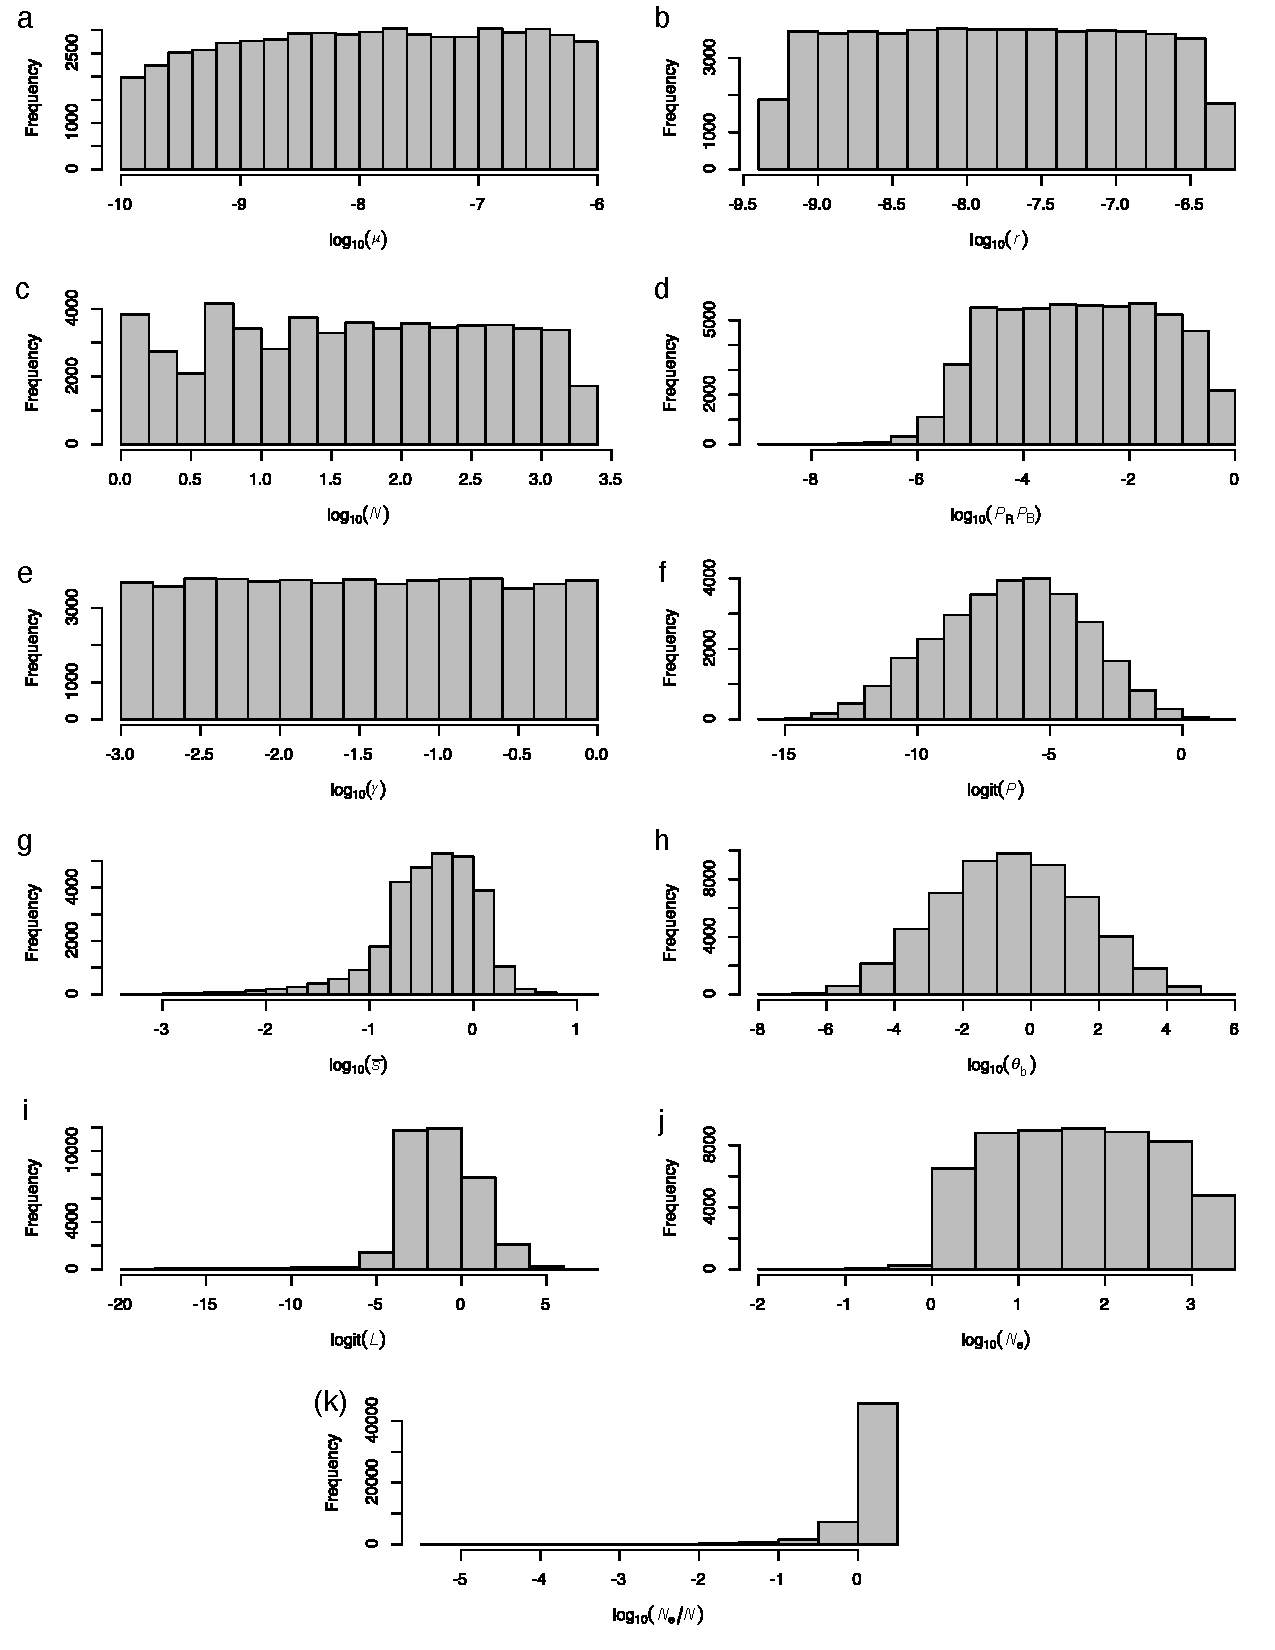
\includegraphics[width=0.85\textwidth]{Figures/supplement/FigureS1_parameters_histograms.pdf}
  \small\caption{\textbf{Prior distribution of the simulation parameters, latent variables informative about the adaptive history and demography inferred with the ABC-RF.} (a) the per site mutation rate $\mu$, (b)  per base recombination rate per generation $c_{\mathrm{0}}$, (c) the population size $N$, (d) the probability of beneficial mutation $P_RP_B$, (e) mean of the gamma distribution $\gamma$, (f) the proportion of strongly selected mutations $P$, (g) average selection coefficients of mutations under strong selection $\bar{s}$, (h) the scale mutation rate of beneficial mutations $\theta_{\mathrm{b}}$, (i) the average substitution load $L$, (j) the effective population size $N_{\mathrm{e}}$, (k) the distance between the effective size and population size expressed in the ratio $N_{\mathrm{e}}/N$.}
  \label{fig:supple_pods_priors}
\end{figure}

% Figure Supplementary 2 - PODs OOB plots << selection >>
\begin{figure}[ht]
  \centering
  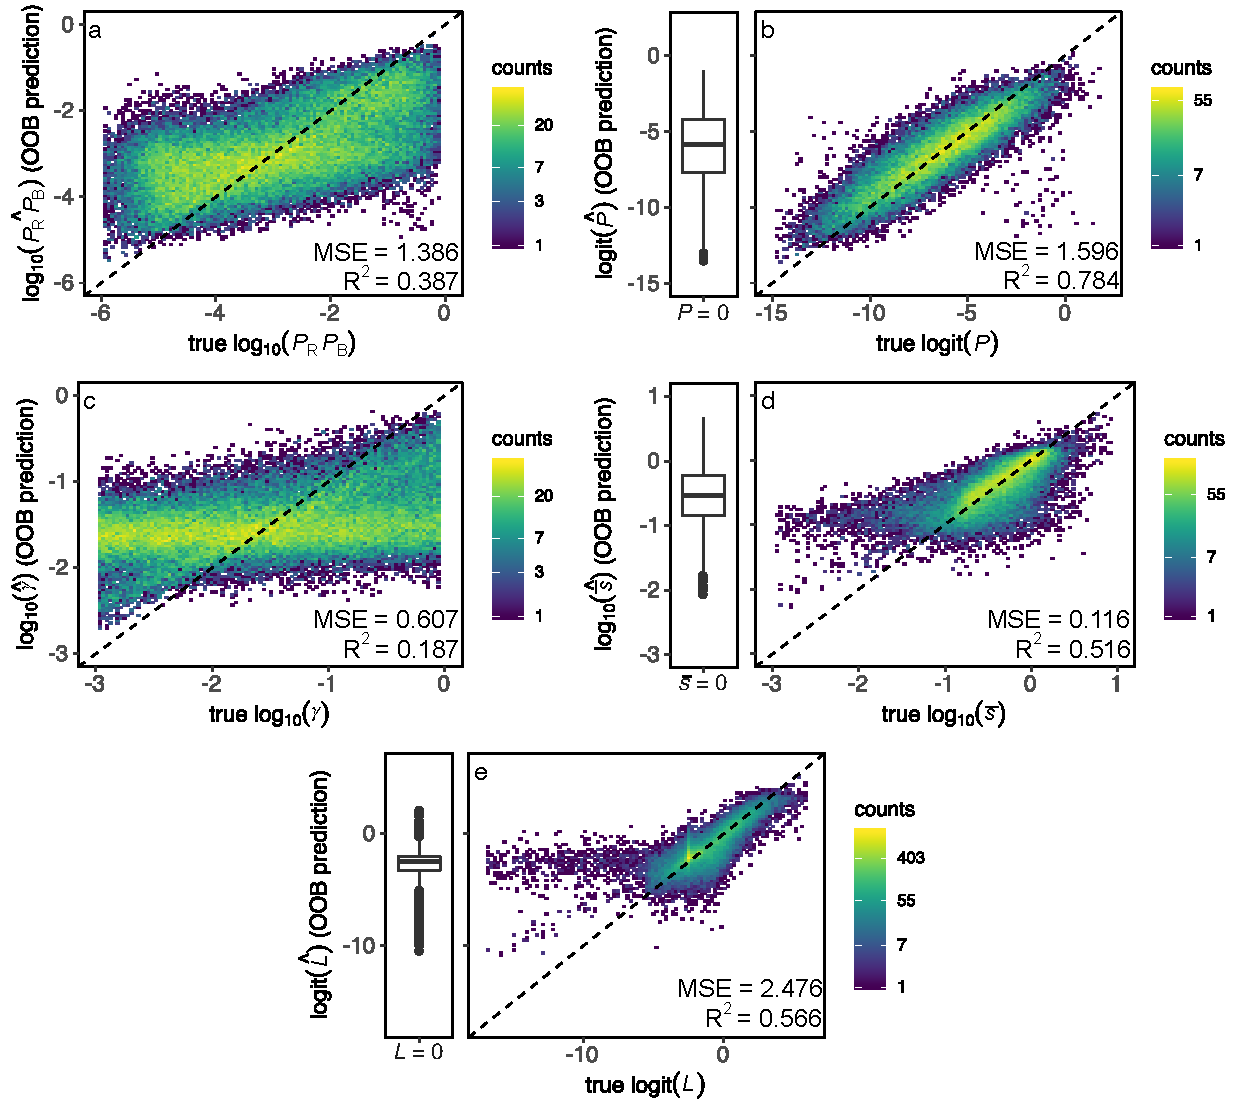
\includegraphics[width=1\textwidth]{Figures/supplement/FigureS2_oob_plots_selection.pdf}
  \small\caption{\textbf{Out-of-bag estimates of ABC-RF trained for the prediction of model parameters informative about the number of beneficial mutations and their strength, the latent variables associated with these two parameters, and variables informative about the adaptive dynamic.} (a) probability of a beneficial mutation to arise $P_RP_B$; (b) number of mutations under strong selection $P$; (c)  mean of the gamma distribution $\gamma$; (d) mean of selection coefficients of mutations under strong selection $\bar{s}$; and (e) mean substitution load $L$. The barplots on the left side of the scatterplots of $P$, $\bar{s}$, and $L$ correspond to the posterior estimates obtained for the simulations removed for the training of these parameters, as these simulations had zero as true values.}
  \label{fig:supple_oob_sel}
\end{figure}

% Figure Supplementary 3 - PODs OOB plots << demography >>
\begin{figure}[ht]
  \centering
  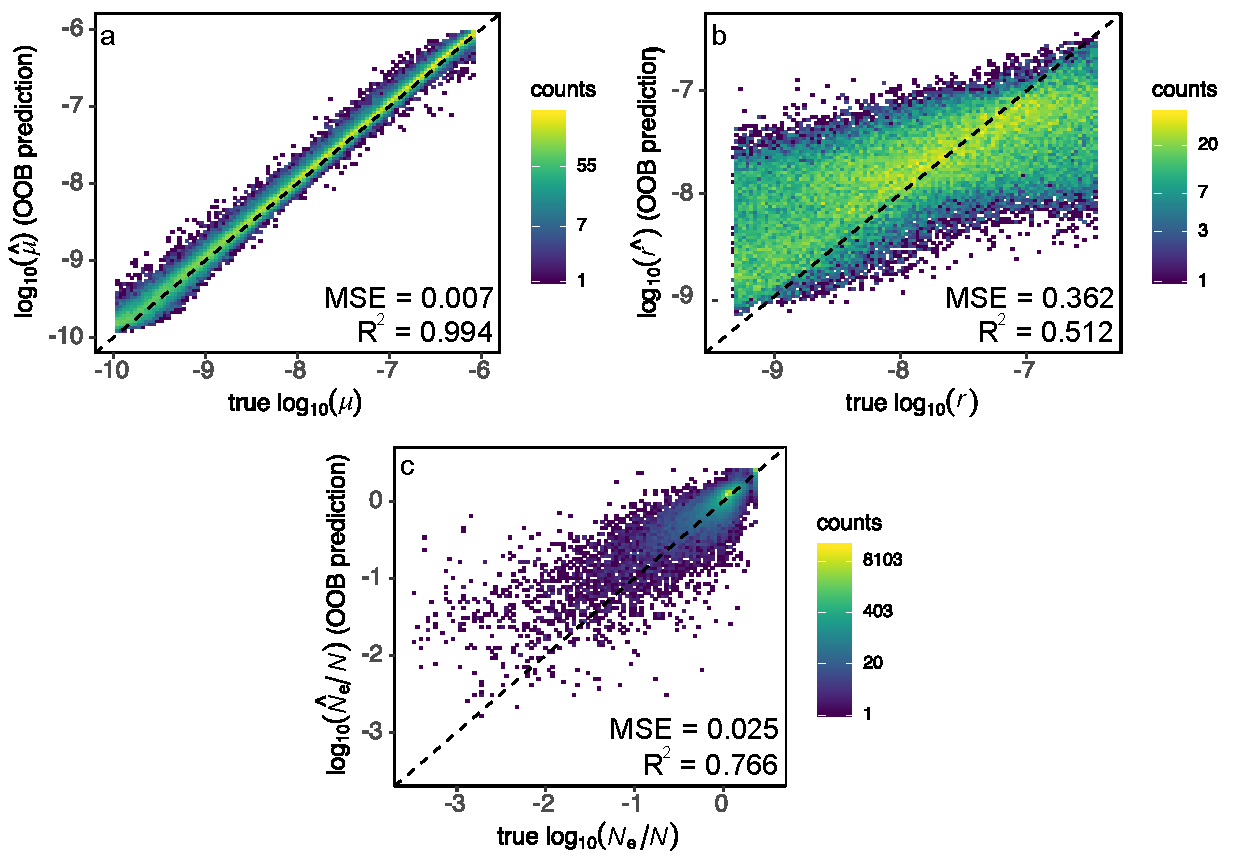
\includegraphics[width=1\textwidth]{Figures/supplement/FigureS3_oob_plots_demography.pdf}
  \small\caption{\textbf{Out-of-bag estimates of ABC-RF trained for the prediction of model parameters and latent variables informative about demography.} (a) mutation rate per generation $\mu$; (b) per base recombination rate per generation $c_{\mathrm{0}}$; and (c) the ratio between the effective size and the population census size $N_{\mathrm{e}}/N$}\label{fig:supple_oob_demo}
\end{figure}

% Figure Supplementary 4 - Variable importance plots - PODs selection parameters
\begin{figure}[ht]
  \centering
  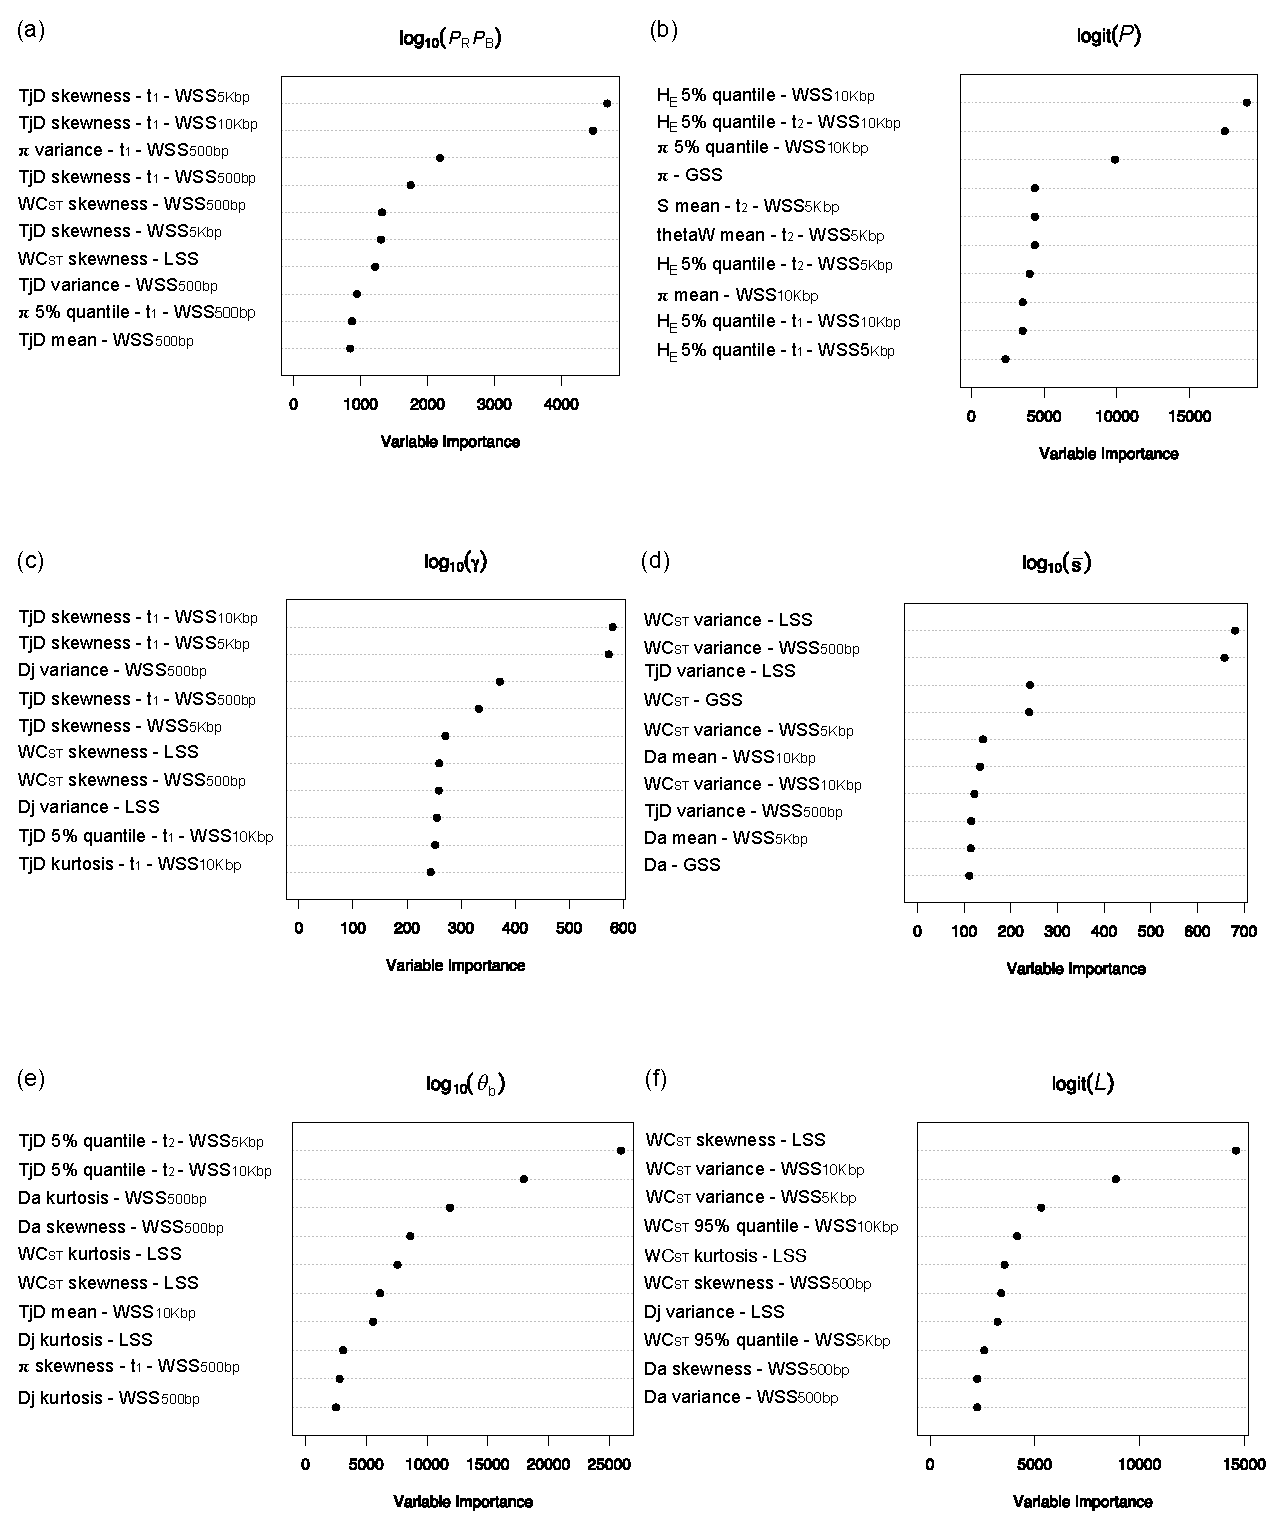
\includegraphics[width=0.95\textwidth]{Figures/supplement/FigureS4_varplot_selection.pdf}
  \small\caption{\textbf{Variable importance plots of the trained ABC-RF for parameters informative about the adaptive history.} (a) The probability of beneficial mutation $P_RP_B$, (b) the proportion of strongly selected mutations $P$, (c) mean of the gamma distribution $\gamma$, (d) average selection coefficients of mutations under strong selection $\bar{s}$, (e) the scale mutation rate of selected mutations $\theta_{\mathrm{b}}$, and (f) the average substitution load $L$.}
  \label{fig:supple_pods_varplots_sel}
\end{figure}

% Figure Supplementary 5 - Variable importance plots - PODs demography parameters
\begin{figure}[ht]
  \centering
  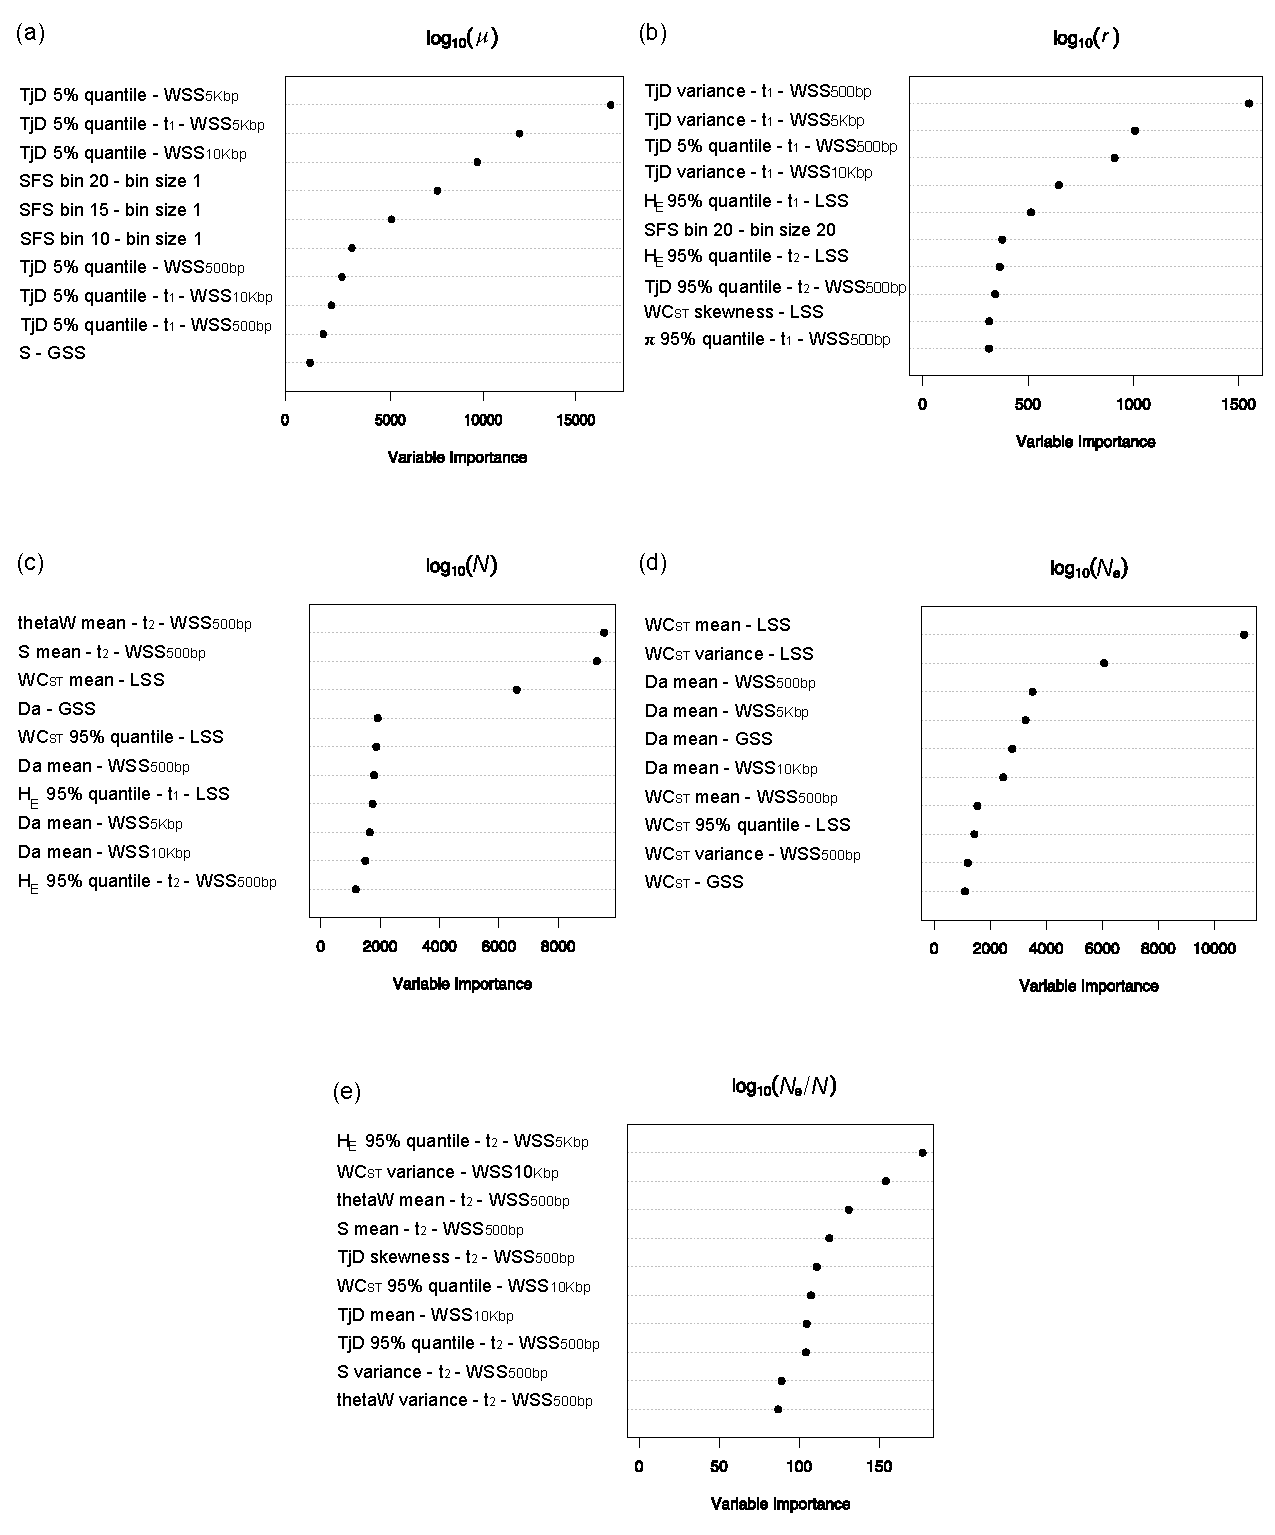
\includegraphics[width=0.95\textwidth]{Figures/supplement/FigureS5_varplot_demography.pdf}
  \small\caption{\textbf{Variable importance plots of the trained ABC-RF for parameters informative about the adaptive history.} (a) the per site mutation rate $\mu$, (b) per base recombination rate per generation $c_{\mathrm{0}}$, (c) the population size $N$, (d) the effective population size $N_{\mathrm{e}}$, (e) the distance between the effective size and population size expressed in the ratio $N_{\mathrm{e}}/N$.}
  \label{fig:supple_pods_varplots_demo}
\end{figure}

% Figure Supplementary 6, 7 and 8 - Feral Bees OOB plots << selection >>
\begin{figure}[ht]
  \centering
  \includegraphics[width=0.95\textwidth]{Figures/supplement/FigureS6_thetab.pdf}
  \small\caption{\textbf{Out-of-bag estimates of ABC-RF trained for the prediction of the scaled mutation rate of beneficial mutations $\theta_{b}$ for pairs of temporal samples of \textit{A. mellifera} feral populations.}}
  \label{fig:supple_feralbee_thetab}
\end{figure}

\begin{figure}[ht]
  \centering
  \includegraphics[width=0.95\textwidth]{Figures/supplement/FigureS7_logn.pdf}
  \small\caption{\textbf{Out-of-bag estimates of ABC-RF trained for the prediction of the population census size $N$ for pairs of temporal samples of \textit{A. mellifera} feral populations.}}
  \label{fig:supple_feralbee_N}
\end{figure}

\begin{figure}[ht]
  \centering
  \includegraphics[width=0.95\textwidth]{Figures/supplement/FigureS8_logmeanNe2.pdf}
  \small\caption{\textbf{Out-of-bag estimates of ABC-RF trained for the prediction of the population effective size $N_{\mathrm{e}}$ for pairs of temporal samples of \textit{A. mellifera} feral populations.}}
  \label{fig:supple_feralbee_NE}
\end{figure}

% Figure Supplementary 9, 10, 11, 12, and 13 - Feral Bees OOB plots << selection extra >>
\begin{figure}[ht]
  \centering
  \includegraphics[width=0.95\textwidth]{Figures/supplement/FigureS9_logP_RP_B.pdf}
  \small\caption{\textbf{Out-of-bag estimates of ABC-RF trained for the prediction of the probability of beneficial mutation $P_RP_B$ for pairs of temporal samples of \textit{A. mellifera} feral populations.}}
  \label{fig:supple_feralbee_prpb}
\end{figure}

\begin{figure}[ht]
  \centering
  \includegraphics[width=0.95\textwidth]{Figures/supplement/FigureS10_logitpopstrongmsel.pdf}
  \small\caption{\textbf{Out-of-bag estimates of ABC-RF trained for the prediction of the proportion of strongly selected mutations $P$ for pairs of temporal samples of \textit{A. mellifera} feral populations.} Stacked points on the far left of each scatter-plot correspond to posterior estimates of neutral simulations, where $P = 0$.}
  \label{fig:supple_feralbee_pstrong}
\end{figure}

\begin{figure}[ht]
  \centering
  \includegraphics[width=0.95\textwidth]{Figures/supplement/FigureS11_loggammamean.pdf}
  \small\caption{\textbf{Out-of-bag estimates of ABC-RF trained for the prediction of the mean of the gamma distribution $\gamma$ for pairs of temporal samples of \textit{A. mellifera} feral populations.}}
  \label{fig:supple_feralbee_gammamean}
\end{figure}

\begin{figure}[ht]
  \centering
  \includegraphics[width=0.95\textwidth]{Figures/supplement/FigureS12_logpopstrongselmean.pdf}
  \small\caption{\textbf{Out-of-bag estimates of ABC-RF trained for the prediction of the average selection coefficients of mutations under strong selection $\bar{s}$ for pairs of temporal samples of \textit{A. mellifera} feral populations.} Stacked points on the far left of each scatter-plot correspond to posterior estimates of neutral simulations, where $\bar{s} = 0$.}
  \label{fig:supple_feralbee_gammaselmean}
\end{figure}

\begin{figure}[ht]
  \centering
  \includegraphics[width=0.95\textwidth]{Figures/supplement/FigureS13_averageGenLoad.pdf}
  \small\caption{\textbf{Out-of-bag estimates of ABC-RF trained for the prediction of the mean substitution load $L$ for pairs of temporal samples of \textit{A. mellifera} feral populations.} Stacked points on the far left of each scatter-plot correspond to posterior estimates of neutral simulations, where $L = 0$.}
  \label{fig:supple_feralbee_load}
\end{figure}

% Figure Supplementary 14, 15, and 16 - Feral Bees OOB plots << demography extra >>
\begin{figure}[ht]
  \centering
  \includegraphics[width=0.95\textwidth]{Figures/supplement/FigureS14_logmu.pdf}
  \small\caption{\textbf{Out-of-bag estimates of ABC-RF trained for the mutation rate per generation $\mu$ for pairs of temporal samples of \textit{A. mellifera} feral populations.}}
  \label{fig:supple_feralbee_mu}
\end{figure}

\begin{figure}[ht]
  \centering
  \includegraphics[width=0.95\textwidth]{Figures/supplement/FigureS15_logrr.pdf}
  \small\caption{\textbf{Out-of-bag estimates of ABC-RF trained for the per base recombination rate per generation $c_{\mathrm{0}}$ for pairs of temporal samples of \textit{A. mellifera} feral populations.}}
  \label{fig:supple_feralbee_c0}
\end{figure}

\begin{figure}[ht]
  \centering
  \includegraphics[width=0.95\textwidth]{Figures/supplement/FigureS16_logmeanNe2ncs.pdf}
  \small\caption{\textbf{Out-of-bag estimates of ABC-RF trained for the the ratio between the effective size and the population census size for pairs of temporal samples of \textit{A. mellifera} feral populations.}}
  \label{fig:supple_feralbee_nen}
\end{figure}

% Figure Supplementary 17 and 18 - Feral Bees Posterior density plots << selection and demography extra >>

\begin{figure}[ht]
  \centering 
  \includegraphics[width=0.95\textwidth]{Figures/supplement/FigureS17_weighted_densityPlots_selection_feralbees.pdf}
  \small\caption{\textbf{Posterior distributions of model parameters and a latent variable informative about selection for all feral \textit{A. mellifera} populations.} (a) probability of a beneficial mutation to arise $P_RP_B$; (b) number of mutations under strong selection $P$; (c)  mean of the gamma distribution $\gamma$; (d) mean of selection coefficients of mutations under strong selection $\bar{s}$; and (e) mean substitution load $L$.}
  \label{fig:supple_feralbee_densityselection}
\end{figure}

\begin{figure}[ht]
  \centering
  \includegraphics[width=0.95\textwidth]{Figures/supplement/FigureS18_weighted_densityPlots_demography_feralbees.pdf}
  \small\caption{\textbf{Posterior distributions of model parameters and a latent variable informative about demography for all feral \textit{A. mellifera} populations.} (a) mutation rate per generation $\mu$; (b) per base recombination rate per generation $c_{\mathrm{0}}$; and (c) the ratio between the effective size and the population census size $N_{\mathrm{e}}/N$.}
  \label{fig:supple_feralbee_densitydemo}
\end{figure}

\end{document}
